\sekshun{Rectangle Integration}
\label{Rectangle_Integration}
\index{rectangle integration}
\index{integration!rectangle}

The rectangle method computes an approximation to a 
definite integral by finding the area of a collection of rectangles whose heights are determined 
by the values of the function.  Specifically, the interval $[a,b]$ over which the function is to 
be integrated is divided into $N$ equal subintervals of length $h = (b-a)/N$. The rectangles are 
drawn with one base along the $x$-axis. Depending on whether the method is left, right, or midpoint,
the left corner, right corner, or midpoint, respectively, of the side opposite the base lies on the 
graph of the function. The approximation to the integral is 
then calculated by adding up the areas (base multiplied by height) of the $N$ rectangles, 
giving the formula:
\begin{equation}
  \int_a^b f(x) dx \approx h \sum_{n=0}^{N-1} f(x_n) \label{eq:rectangle}
\end{equation}
where
\begin{equation}
  h=(b-a)/N  \label{eq:subinterval-width}
\end{equation}

The formula for $x_n$ for the left, right, and midpoint methods are given in Table \ref{tab:xn-rectangle}.
As $N$ gets larger, the rectangle method becomes more accurate. This is illustrated in the series of plots
in Figure \ref{fig:rectangle}.

\begin{table}[htbp]
  \centering
  \caption{Formula for $x_n$ in Equation \ref{eq:rectangle} of 
  rectangle numerical integration methods.} 
  \label{tab:xn-rectangle}
  \begin{tabular}{cc}
    \textbf{Method} & \textbf{$x_n$} \\ \toprule
    left & $a+nh$ \\ \midrule
    right & $a+(n+1)h$ \\ \midrule
    midpoint & $a+\left(n + \frac{1}{2}\right)h$ \\ \bottomrule
  \end{tabular}
\end{table}

\begin{figure}
  \centering
  \subcaptionbox{$N=4$}{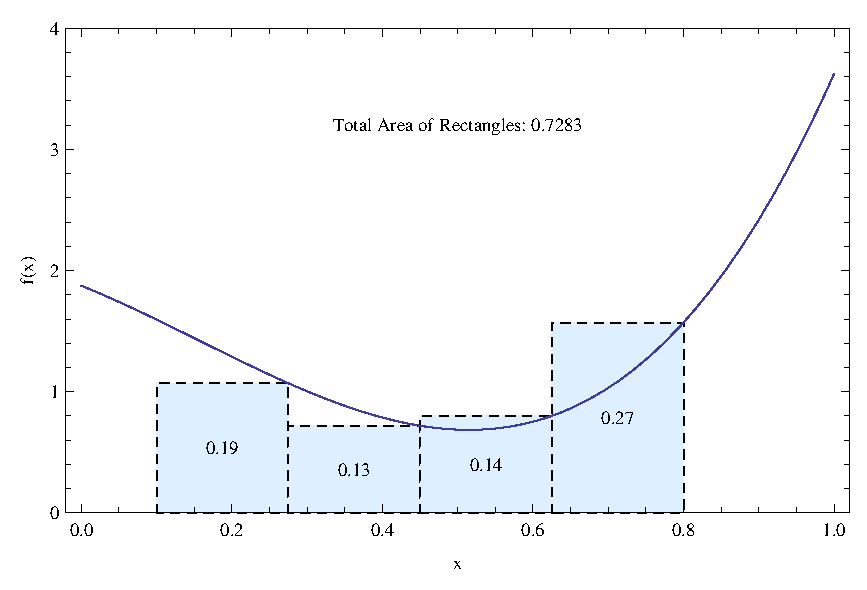
\includegraphics[scale=.6]{fig/rightrectangle-4.eps}}
  \subcaptionbox{$N=6$}{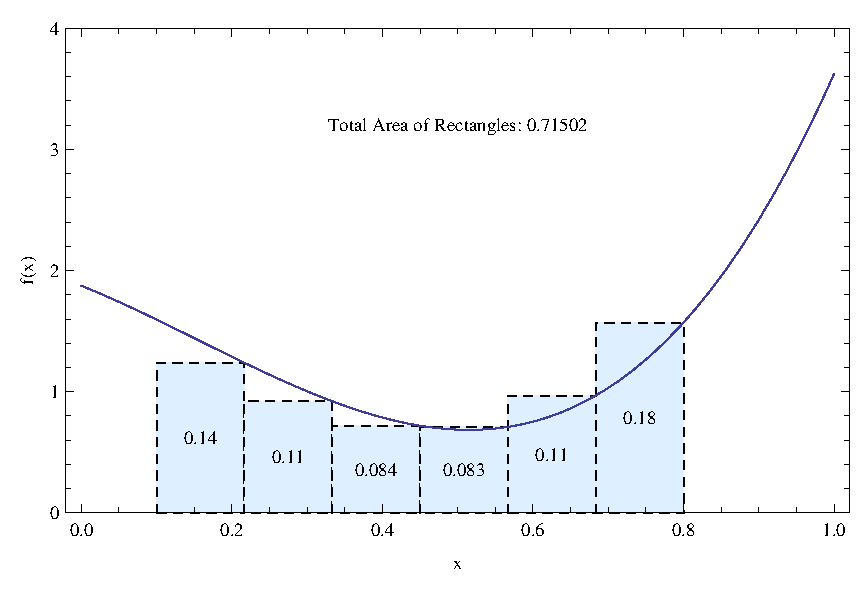
\includegraphics[scale=.6]{fig/rightrectangle-6.eps}}
  \subcaptionbox{$N=10$}{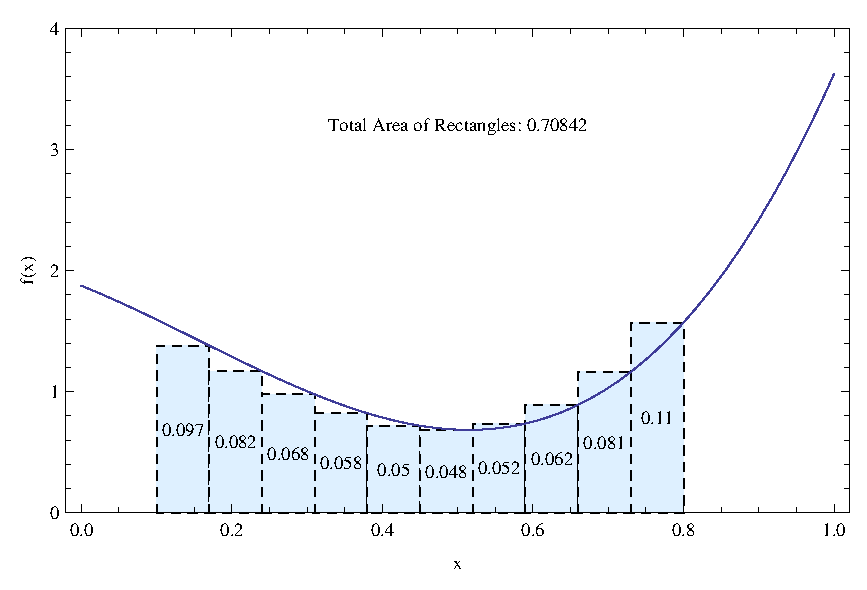
\includegraphics[scale=.6]{fig/rightrectangle-10.eps}}
  \caption{Numerical integration of $f(x) = (2 x-0.5)^3+(1.5 x-1)^2-x+1$ for $x$ in $[0.1,0.8]$
    by the (right) rectangle method for increasing values of $N$. The number inside each rectangle is
    the area of that rectangle, and the total area is displayed on each graph.
  The exact value of the integral is 0.70525.}\label{fig:rectangle}
\end{figure}

\section{Left Rectangle Method}
\begin{seamlessnote}
  Now that we've described the rectangle methods fairly well, we will begin developing the code 
  for the left rectangle version.  The first step is to develop the tests, and
  every test needs an expected value against which to compare. For our cases, we have the exact
  values for the integrals, but exact values alone are insufficient to test numerical methods
  against. We need to understand by how much the output from our functions can deviate from
  the exact values. Fortunately, the maximum error expressions for these methods are well
  known.
\end{seamlessnote}

If $f(x)$ is increasing or decreasing on the interval $[a,b]$, the maximum error $E$ 
for left or right rectangular numerical integration is given by
\begin{equation}
  E \leq \frac{b-a}{N}\left|f(b)-f(a)\right| \label{eq:lr-rectangle-max-error}
\end{equation}

We can create a helper function to compute the maximum error for left and right rectangle
methods using Equation~\ref{eq:lr-rectangle-max-error}. The calculated value will be used
in tests for the left and right rectangle methods to check that the result is within 
the maximum error expected for a given $a$, $b$, and $N$. 
\begin{enumspec}
\item\spec{1} Helper function \lstinline{leftRightRectangleMaxErr} returns the
  maximum error expected for left or right rectangle method numerical integration. It 
  takes in a reference to a pre-defined function $f$, the bounds $a$ (real) and $b$ (real) of the 
  interval for definite integration, and the number $N$ (integer) of subintervals used.
  The function will be entered in \lstinline{leftRightRectangleMaxErr.chpl}.
  \meetsreq{5,5.1}
\end{enumspec}

\begin{chapelhelper}{leftRightRectangleMaxErr.chpl}
  \begin{chapel}
    proc leftRightRectangleMaxErr(a: real, b: real, N: int, f): real{
      return ((b-a)/N)*abs(f(b)-f(a));
    }
  \end{chapel}
\end{chapelhelper}

\begin{seamlessnote}
  In \lstinline{seamless} vernacular, the helper files are chunks of code that are used to support
  testing that the developer wants to have outside of the tests. The most likely reason being that
  the code contains setup or auxiliary functions that are used for multiple tests. In our example
  above, we are using some foresight and envisioning that the \lstinline{leftRightRectangleMaxErr}
  function will also be used in a test for the left rectangle numerical integration function. To 
  extract the helper files from your latex source files, run the following command in the same
  directory as your latex source:
  \begin{verbatim}
  [./tutorial/] $ make helpers
  \end{verbatim}
  This command runs the \lstinline{helpers} target in the Makefile at the root of the 
  tutorial directory (\lstinline{./tutorial/Makefile}. A Makefile is a text 
    file written in a certain prescribed syntax. Together with the \lstinline{make} utility, it 
    helps automate repetitive commandline tasks such as building software from its source files. 
    In this case, the \lstinline{helpers} target cleans out the \lstinline{./tutorial/helper} directory and
    executes the \lstinline{./util/extract\_helpers} python script with the appropriate arguments.
  \end{seamlessnote}

  One of the functions that we need to test our methods against is $f(x) = x^3$, 
  with $a=0$, $b=1$, and $N=100$.
  Since the function is increasing on the interval $[0,1]$, we can use 
  the helper function that we just created to compute the maximum expected error. We are
  ready to create our first test for a function that we will write to compute the definite
  integral using the left rectangle method. This function will be called 
  \lstinline{leftRectangleIntegration}
  and will be written to \lstinline{leftRectangleIntegration.chpl}.
  Since we know we have four tests to construct (Requirements \ref{req5.1} through \ref{req5.4}),
  we will label the specification for this first test \ref{spec2.1}
  \begin{TODO}
    Add seamless note on how to reference spec's and req's.
  \end{TODO}

  \begin{enumspec}
  \item\spec{2.1}
    Test \lstinline{leftRectangleIntegrationTest1.chpl} loads modules
    \lstinline{leftRightRectangleMaxErr} and
    \lstinline{leftRectangleIntegration}.
    It defines a function \lstinline{f} that takes $x$ (real) and returns $x^3$ (real).
    It passes $a=0.0$, $b=1.0$, $N=100$, and \lstinline{f} to the function
    \lstinline{leftRightRectangleMaxErr} and stores the result in the variable
    \lstinline{maximumError} (real).
    It passes $a=0.0$, $b=1.0$, $N=100$, and \lstinline{f} to the function
    \lstinline{leftRectangleIntegration} and stores the result in the variable
    \lstinline{calculated}.
    Variable \lstinline{exact: real} is initialized with the exact value of the integral from
    Mathematica, 0.25.
    It then checks to see if the absolute value of the difference between \lstinline{calculated} 
    and \lstinline{exact} is less than or equal to \lstinline{maximumError} and sets 
    \lstinline{verified: bool}. The test writes out \lstinline{verified} and a passing
    test results in \lstinline{true}.
    \meetsreq{5.1}
  \end{enumspec}

  \begin{chapelexample}{leftRectangleIntegrationTest1.chpl}
    A test for \lstinline{leftRectangleIntegration}.
    \begin{chapelpre}
    \end{chapelpre}
    \begin{chapel}
      use leftRightRectangleMaxErr;
      use leftRectangleIntegration;
      proc f(x:real):real {
        return x**3;
      } 

      var calculated:real;
      var exact:real = 0.25;  // from Mathematica
      var maximumError:real = leftRightRectangleMaxErr(a = 0.0, b = 1.0, N = 100, f = f);
      var verified:bool;

      calculated = leftRectangleIntegration(a = 0.0, b = 1.0, N = 100, f = f);
      verified = (abs(calculated - exact) <= maximumError);
      writeln(verified);
    \end{chapel}
    \begin{chapelpost}
    \end{chapelpost}
    \begin{chapeloutput}
true
    \end{chapeloutput}
  \end{chapelexample}

  \begin{seamlessnote}
    Now that we have our first test written, we need to extract it from the latex source and verify
    that it does not pass.
    To extract the test from the latex source and run it:
    \begin{verbatim}
    [./tutorial/] $ make tests
    [./tutorial/] $ make test
    \end{verbatim}
    These commands run the \lstinline{tests} and \lstinline{test} targets in the same Makefile referenced above.
    In this case, the \lstinline{tests} target cleans out the \lstinline{./tutorial/test} directory and
    executes the \lstinline{./util/extract_tests} python script with the appropriate arguments.
    The \lstinline{test} target changes to the \lstinline{./tutorial/test} directory and 
    executes the \lstinline{start_test} csh script that comes with
    the chapel distribution (in \lstinline{CHPL_HOME/util}). The script compiles and executes each of the
    chapel source files in the test directory 
    (\eg \lstinline{leftRectangleIntegrationTest.chpl} as in the example above) 
    and compares the output with the contents of a file with a \lstinline{.good} extension
    (\eg \lstinline{leftRectangleIntegrationTest.good} for the above test). 
    The last few lines of output should look something like this:
    \begin{verbatim}
    [Test Summary - 150107.202408]
    [Summary: #Successes = 0 | #Failures = 1 | #Futures = 0 | #Warnings = 0 ]
    [END]
    \end{verbatim}
  \end{seamlessnote}

  \begin{TODO}
    Update test target to run all targets necessary to run tests.
  \end{TODO}

  The code that provides the \lstinline{leftRectangleIntegration} function is straightforward.
  \begin{enumspec}
  \item\spec{3} Function \lstinline{leftRectangleIntegration}, for an interval
    of integration, $[a,b]$,
    takes the left end value of the interval, \lstinline{a: real}, the right end value
    of the interval, \lstinline{b: real}, the number of subintervals for the numerical
    integration, \lstinline{N: int}, and the function to be integrated, \lstinline{f}.
    The function stores the width of the subinterval calculated from Equation 
    \ref{eq:subinterval-width} in the variable \lstinline{h: real}. It initializes the variable
    \lstinline{sum: real} to zero, and for each value of $n$ in the summation of Equation~\ref{eq:rectangle},
    it computes \lstinline{x_n: real} according to the expression in Table~\ref{tab:xn-rectangle} and adds
    the value of \lstinline{f(x_n)} to \lstinline{sum: real}. The function returns the product of 
    \lstinline{sum: real} and the subinterval width, \lstinline{h: real}.
    \meetsreq{1}
  \end{enumspec}

  \begin{chapelsource}{leftRectangleIntegration.chpl}
    \begin{chapel}
      proc leftRectangleIntegration(a: real(64), b: real(64), N: int(64), f): real(64){
        var h: real(64) = (b - a)/N; 
        var sum: real(64) = 0.0;
        var x_n: real(64);
        for n in 0..N-1 {
          x_n = a + n * h;
          sum = sum + f(x_n);
        }
        return h * sum;
      }
    \end{chapel}
  \end{chapelsource}

  \begin{seamlessnote}
    We can now verify that test \lstinline{leftRectangleIntegrationTest1.chpl} passes. First
    we need to extract the chapel source from our latex file and then run the test that was
    written previously:
    \begin{verbatim}
  [./tutorial/] $ make sources
  [./tutorial/] $ make test
  \end{verbatim}
  These commands run the \lstinline{sources} and \lstinline{test} targets in our Makefile.
  In this case, the \lstinline{sources} target cleans out the \lstinline{./tutorial/source} directory and
  executes the \lstinline{./util/extract_sources} python script with the appropriate arguments, putting
  the source code that we've defined in our latex file into the \lstinline{./tutorial/source} directory.
  The last few lines of output should look something like this:
  \begin{verbatim}
  [Test Summary - 150107.202408]
  [Summary: #Successes = 1 | #Failures = 0 | #Futures = 0 | #Warnings = 0 ]
  [END]
  \end{verbatim}
\end{seamlessnote}

Another of the functions that we need to test our methods against is 
$f(x) = 1/x$, where $x$ is $[1,100]$, with 1,000 approximations. 
The exact result is the natural log of 100, or about 4.605170.
Since the function is decreasing on the interval $[1,100]$, we can again use 
the helper function in \lstinline{leftRightRectangleMaxErr.chpl} to compute the 
maximum expected error.  
Our second test 
for the left rectangle method is very similar to the first. 
\begin{enumspec}
\item\spec{4}
  Test \lstinline{leftRectangleIntegrationTest2.chpl} loads modules
  \lstinline{leftRightRectangleMaxErr} and
  \lstinline{leftRectangleIntegration}.
  It defines a function \lstinline{f} that takes \lstinline{x: real} and returns $1/x$.
  It passes $a=1.0$, $b=100.0$, $N=1000$, and \lstinline{f} to the function
  \lstinline{leftRightRectangleMaxErr} and stores the result in the variable
  \lstinline{maximumError} (real).
  It passes $a=1.0$, $b=100.0$, $N=1000$, and \lstinline{f} to the function
  \lstinline{leftRectangleIntegration} and stores the result in the variable
  \lstinline{calculated}.
  Variable \lstinline{exact: real} is initialized with the exact value of the integral, 4.605170.
  It then checks to see if the absolute value of the difference between \lstinline{calculated} 
  and \lstinline{exact} is less than or equal to \lstinline{maximumError} and sets 
  \lstinline{verified: bool}. The test writes out \lstinline{verified} and a passing
  test results in \lstinline{true}.
  \meetsreq{5.2}
\end{enumspec}

\begin{chapelexample}{leftRectangleIntegrationTest2.chpl}
  A test for \lstinline{leftRectangleIntegration} using $f(x) = 1/x$.
  \begin{chapelpre}
  \end{chapelpre}
  \begin{chapel}
    use leftRightRectangleMaxErr;
    use leftRectangleIntegration;

    proc f(x:real):real {
      return 1/x;
    } 

    var exact:real = 4.605170; 
    var maximumError:real = leftRightRectangleMaxErr(a = 1.0, b = 100.0, N = 1000, f = f);
    var calculated: real = leftRectangleIntegration(a = 1.0, b = 100.0, N = 1000, f = f);
    var verified: bool = (abs(calculated - exact) <= maximumError);
    writeln(verified);
  \end{chapel}
  \begin{chapelpost}
  \end{chapelpost}
  \begin{chapeloutput}
true
  \end{chapeloutput}
\end{chapelexample}

\begin{seamlessnote}
  By now you have likely realized that we already have some opportunities to refactor code in
  our first two tests above. The tests are very similar except for the expressions in the 
  test function ($f$), the exact values for the integrals, and the values of $a$, $b$, and $N$
  passed to \lstinline{leftRightRectangleMaxErr} and \lstinline{leftRectangleIntegration}.
  Also, you'll notice that the arguments to 
  \lstinline{leftRightRectangleMaxErr} and \lstinline{leftRectangleIntegration}
  are identical, and perhaps it would be good to always get the maximum error associated with a
  numerical integration.
  We will rewrite our integration function to return the value of the integral and
  the maximum error in a tuple. 
  We can also combine the two tests and add the final two tests using the function $f(x) = x$.
  In practice, the developer would typically not keep the above two tests. She would 
  replace the above two tests with what follows and the resulting \lstinline{seamless} 
  document would be much more streamlined than what is presented here. Of course, there is no 
  harm in keeping all of the versions of the tests.
\end{seamlessnote}

\begin{TODO}
  Add description of versioning with git.
\end{TODO}

\begin{chapelexample}{leftRectangleIntegrationTest3.chpl}
  A test for \lstinline{leftRectangleIntegration} using $f(x) = \{x^3, 1/x, x\}$.
  \begin{chapelpre}
  \end{chapelpre}
  \begin{chapel}
    use leftRectangleIntegrationWithErr;

    proc f1(x:real):real {
      return x**3;
    } 
    proc f2(x:real):real {
      return 1/x;
    } 
    proc f3(x:real):real {
      return x;
    } 

    var exact:real;
    var calculated:real;
    var maxErr:real;

    exact = 0.25;
    (maxErr, calculated) = leftRectangleIntegrationWithErr(a = 0.0, b = 1.0, N = 100, f = f1);
    writeln((abs(calculated - exact) <= maxErr));

    exact = 4.605170;
    (maxErr, calculated) = leftRectangleIntegrationWithErr(a = 1.0, b = 100.0, N = 1000, f = f2);
    writeln((abs(calculated - exact) <= maxErr));

    exact = 12500000;
    (maxErr, calculated) = leftRectangleIntegrationWithErr(a = 0.0, b = 5000.0, N = 5000000, f = f3);
    writeln((abs(calculated - exact) <= maxErr));

    exact = 18000000;
    (maxErr, calculated) = leftRectangleIntegrationWithErr(a = 0.0, b = 6000.0, N = 6000000, f = f3);
    writeln((abs(calculated - exact) <= maxErr));
  \end{chapel}
  \begin{chapelpost}
  \end{chapelpost}
  \begin{chapeloutput}
true
true
true
true
  \end{chapeloutput}
\end{chapelexample}

The code that provides the \lstinline{leftRectangleIntegrationWithErr} function is straightforward.
\begin{enumspec}
\item\spec{5} Function \lstinline{leftRectangleIntegrationWithErr}, for an interval
  of integration, $[a,b]$,
  takes the left end value of the interval, \lstinline{a: real}, the right end value
  of the interval, \lstinline{b: real}, the number of subintervals for the numerical
  integration, \lstinline{N: int}, and the function to be integrated, \lstinline{f}.
  The function stores the width of the subinterval calculated from Equation 
  \ref{eq:subinterval-width} in the variable \lstinline{h: real}. It initializes the variable
  \lstinline{sum: real} to zero, and for each value of $n$ in the summation of Equation~\ref{eq:rectangle},
  it computes \lstinline{x_n: real} according to the expression in Table~\ref{tab:xn-rectangle} and adds
  the value of \lstinline{f(x_n)} to \lstinline{sum: real}. The function returns the product of 
  \lstinline{sum: real} and the subinterval width, \lstinline{h: real} as the first element of a two-element
  tuple..
  The second element of the returned tuple is the
  maximum error expected calculated according to equation \ref{eq:lr-rectangle-max-error}.  \meetsreq{1,5,5.1}
\end{enumspec}

\begin{chapelsource}{leftRectangleIntegrationWithErr.chpl}
  \begin{chapel}
    proc leftRectangleIntegrationWithErr(a: real(64), b: real(64), N: int(64), f): 2*real{
      var maxErr: real = ((b-a)/N)*abs(f(b)-f(a));
      var h: real(64) = (b - a)/N; 
      var sum: real(64) = 0.0;
      var x_n: real(64);
      for n in 0..N-1 {
        x_n = a + n * h;
        sum = sum + f(x_n);
      }
      return (h * sum, maxErr);
    }
  \end{chapel}
\end{chapelsource}

\section{Right Rectangle Method}

\begin{chapelexample}{rightRectangleIntegrationTest.chpl}
  A test for \lstinline{rightRectangleIntegrationWithErr} using $f(x) = \{x^3, 1/x, x\}$.
  \begin{chapelpre}
  \end{chapelpre}
  \begin{chapel}
    use rightRectangleIntegrationWithErr;

    proc f1(x:real):real {
      return x**3;
    } 
    proc f2(x:real):real {
      return 1/x;
    } 
    proc f3(x:real):real {
      return x;
    } 

    var exact:real;
    var calculated:real;
    var maxErr:real;

    exact = 0.25;
    (maxErr, calculated) = rightRectangleIntegrationWithErr(a = 0.0, b = 1.0, N = 100, f = f1);
    writeln((abs(calculated - exact) <= maxErr));

    exact = 4.605170;
    (maxErr, calculated) = rightRectangleIntegrationWithErr(a = 1.0, b = 100.0, N = 1000, f = f2);
    writeln((abs(calculated - exact) <= maxErr));

    exact = 12500000;
    (maxErr, calculated) = rightRectangleIntegrationWithErr(a = 0.0, b = 5000.0, N = 5000000, f = f3);
    writeln((abs(calculated - exact) <= maxErr));

    exact = 18000000;
    (maxErr, calculated) = rightRectangleIntegrationWithErr(a = 0.0, b = 6000.0, N = 6000000, f = f3);
    writeln((abs(calculated - exact) <= maxErr));
  \end{chapel}
  \begin{chapelpost}
  \end{chapelpost}
  \begin{chapeloutput}
true
true
true
true
  \end{chapeloutput}
\end{chapelexample}

\begin{chapelsource}{rightRectangleIntegrationWithErr.chpl}
  \begin{chapel}
    proc rightRectangleIntegrationWithErr(a: real(64), b: real(64), N: int(64), f): 2*real{
      var maxErr: real = ((b-a)/N)*abs(f(b)-f(a));
      var h: real(64) = (b - a)/N; 
      var sum: real(64) = 0.0;
      var x_n: real(64);
      for n in 0..N-1 {
        x_n = a + (n + 1) * h;
        sum = sum + f(x_n);
      }
      return (h * sum, maxErr);
    }
  \end{chapel}
\end{chapelsource}

\section{Midpoint Rectangle Method}
For a function $f$ which is twice differentiable, the maximum error $E$ for the
midpoint rectangle method is given by the following equation:
\begin{equation}
  E \leq \frac{(b-a)^3}{24 N^2} f''(\xi) \label{eq:rectangle-max-error}
\end{equation}
for some $\xi$ in $[a,b]$.

Unlike the left and right rectangle methods, it is very difficult to write a function
to determine the maximum expected error. First, we must determine the maximum value of
the second derivative before we can compute the maximum error using 
Equation~\ref{eq:rectangle-max-error}. 
For $f(x) = x^3$, the second derivative is $f''(x) = 6x$. On the interval specified by
Requirement~\ref{req@5.1}, $[0,1]$, the maximum value is $f''(1) = 6$.
For $f(x) = 1/x$, the second derivative is $f''(x) = 2x^{-3}$. On the interval specified by
Requirement~\ref{req@5.2}, $[1,100]$, the maximum value is $f''(1) = 2$.
The function $f(x) = x$ specified by Requirement~\ref{req@5.3} and \ref{req@5.4}, does not have
a second derivative. The midpoint method is expected to give a very accurate answer for this function,
so we will use a value of 0.000001 for the maximum expected error for the two final tests.
The calculated maximum expected error for the tests specified in Requirements~\ref{req@5.1} and
\ref{req@5.2} are given in Table~\ref{tab:midpoint-rectangle-error}.

\begin{table}[htbp]
  \centering
  \caption{Values for expressions in Equation~\ref{eq:rectangle-max-error} and the maximum 
    expected error of the midpoint rectangle method of numerical integration for three
  different functions.}
  \label{tab:midpoint-rectangle-error}
  \begin{tabular}{ccccc}
    \textbf{Function} & \textbf{Interval} & \textbf{N} & \textbf{Maximum $f''(x)$} & $E$  \\ \toprule
    $x^3$ & $[0,1]$   & 100  & 6 & 0.000025 \\ \midrule
    $1/x$ & $[1,100]$ & 1000 & 3 & 0.121287 \\ \bottomrule
  \end{tabular}
\end{table}

\begin{chapelexample}{midpointRectangleIntegrationTest.chpl}
  A test for \lstinline{midpointRectangleIntegrationWithErr} using $f(x) = \{x^3, 1/x, x\}$.
  \begin{chapelpre}
  \end{chapelpre}
  \begin{chapel}
    use midpointRectangleIntegrationWithErr;

    proc f1(x:real):real {
      return x**3;
    } 
    proc f2(x:real):real {
      return 1/x;
    } 
    proc f3(x:real):real {
      return x;
    } 

    var exact:real;
    var calculated:real;
    var maxErr:real;

    exact = 0.25;
    maxErr = 0.000025;
    calculated = midpointRectangleIntegrationWithErr(a = 0.0, b = 1.0, N = 100, f = f1);
    writeln((abs(calculated - exact) <= maxErr));

    exact = 4.605170;
    maxErr = 0.121287;
    calculated = midpointRectangleIntegrationWithErr(a = 1.0, b = 100.0, N = 1000, f = f2);
    writeln((abs(calculated - exact) <= maxErr));

    exact = 12500000;
    maxErr = 0.000001;
    calculated = midpointRectangleIntegrationWithErr(a = 0.0, b = 5000.0, N = 5000000, f = f3);
    writeln((abs(calculated - exact) <= maxErr));

    exact = 18000000;
    maxErr = 0.000001;
    calculated = midpointRectangleIntegrationWithErr(a = 0.0, b = 6000.0, N = 6000000, f = f3);
    writeln((abs(calculated - exact) <= maxErr));
  \end{chapel}
  \begin{chapelpost}
  \end{chapelpost}
  \begin{chapeloutput}
true
true
true
true
  \end{chapeloutput}
\end{chapelexample}

\begin{chapelsource}{midpointRectangleIntegrationWithErr.chpl}
  \begin{chapel}
    proc midpointRectangleIntegrationWithErr(a: real(64), b: real(64), N: int(64), f): real{
      var h: real(64) = (b - a)/N; 
      var sum: real(64) = 0.0;
      var x_n: real(64);
      for n in 0..N-1 {
        x_n = a + (n + 0.5) * h;
        sum = sum + f(x_n);
      }
      return h * sum;
    }
  \end{chapel}
\end{chapelsource}


